\section{Tests et Validation}

\subsection{Introduction}

Afin
d’assurer une stabilité et une fiabilité optimales, nous avons décidé d'effectuer des tests sur les principales classes de l'abstraction. Il s'est agi de tests unitaires pour la plupart des composants (les \verb!Ports! et l'\verb!AudioDeviceProvider!) et le \verb!Sequencer!, qui ont été possibles grâce à la mise en place de bouchons~;
ainsi que des tests fonctionnels pour les modules.
Pour cela, nous avons utilisé le \emph{framework} de tests
unitaires de Qt.

\subsection{WaveGenerator}

\subsubsection{TestWaveGeneratorEmpty}

Avant de tester la génération des ondes sonores, nous avons dû
vérifier qu'une génération simple fonctionnait correctement. Nous
avons donc créé une \verb!WaveGeneratorEmpty!, implémentation de
\verb!WaveGenerator!, qui ne sait que remplir un buffer nul. Ce
test instancie donc ce générateur, lance la génération et vérifie
que buffer de sortie contient bien des 0.

\subsubsection{TestWaveGeneratorSinus, TestWaveGeneratorSquare, TestWaveGeneratorSaw, TestWaveGeneratorTriangle}

Tester que la production d'ondes est correcte n'est pas aisé. On
peut passer par l'étude des signaux générés, mais cela demande un
travail de traitement du signal important qui ne nous paraissait
pas forcément utile, ni très pertinent : l'étude des signaux peut
être bien plus sujette aux erreurs que la génération d'ondes
elle-même.

Notre méthode de test a donc consisté à générer une onde et à la
sauvegarder dans un fichier WAV grâce au module \verb!WavRecorder!.
L'écoute et la visualisation du signal sous un logiciel tel que
Audacity ou Soundforge nous indique si le résultat paraît
conforme.

Nous avons poussé l'étude plus loin en passant les échantillons
sous un accordeur virtuel : la fréquence générée est alors affichée
et il nous est alors possible de savoir si le signal a la fréquence
désirée (figure \ref{fig:accordeur}).

\begin{figure}[htb]
\centering
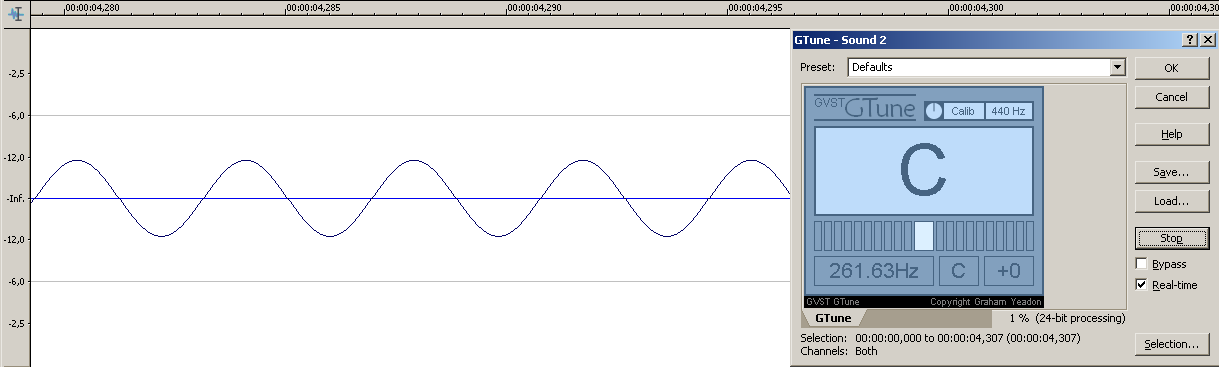
\includegraphics[width=17cm]{../img/png/testWaveGeneratorSinus.png}
\caption{Vérification des ondes générées grace à d'autres logiciels}
\label{fig:accordeur}
\end{figure}

\subsection{VCO}
Pour ce module, nous avons testé :
\begin{itemize}
    \item qu'un onde  carrée demandée au \texttt{WaveGenerator} se retrouvait bien dans le port d'entrée d'un module \textit{mock}. Ce test est effectué en mettant toutes les valeurs du buffer du mock dans un QSet et en constatant qu'au final, il ne contient que deux valeurs et que celles-ci sont opposées~;
    \item que la variation du \texttt{K} d'une unité faisait doubler la fréquence de l'onde obtenue~;
    \item que le sélecteur de forme d'onde sélectionnait effectivement l'onde demandée.
\end{itemize}

\subsection{VCA}
Le rôle du \verb!VCA! étant de multiplier chaque valeur de son entrée par un coefficient, son test a consisté à le faire fonctionner avec un gain donné et à vérifier que les valeurs produites dans un \emph{mock} étaient conformes à nos attentes.

\subsection{VCF}

\subsubsection{Test VCF}

Le test du \verb!VCF! consiste à lier une instance de \verb!VCO! à
un \verb!VCF!. Le VCO ne produira qu'une onde de type \verb!Empty!,
donc ne produisant que des 0. Nous utilisons le filtre
\verb!FilterIncrement! qui se contente d'ajouter 1 à toute valeur
du buffer d'entrée si elle est positive, ou --1 si elle est
négative. Le test s'assure que le buffer de sortie du \verb!VCF! ne
contient que des 1.

\subsubsection{Les filtres}

Il n'est pas facile de tester simplement les filtres. Tout comme
pour les \verb!WaveGenerators!, il faudrait décomposer le signal
afin de tester son intégrité. Cependant, là où la génération
fournie par les \verb!WaveGenerators! pouvait être étudiée par la
suite sous des logiciels tels que Soundforge ou Audacity, il n'en
est pas de même pour les filtres. Nous avons donc décidé de nous fier
à l'écoute du signal et à l’affichage produit par le module Oscilloscope.

\subsection{Test ADSR}

Nous avons testé ce module grâce au fait que son comportement est lié à ce qu'il reçoit dans son port \texttt{gate}. Sur une «~durée~» de trois buffers, nous lui envoyons donc des valeurs 1, puis des zeros, puis des 1, ce qui correspond à un cycle ADSR complet. Les résultats des appels à \texttt{process} sont stockés dans un buffer puis analysés par parcours du dit \emph{buffer} à la recherche de chaque segment du cycle. Les quatres valeurs obtenues sont ensuite comparées à celles données en entrée.


\subsection{Test Mixer}

Le test du Mixer est réalisé en plaçant des buffers constants en entrée de chaque\dots entrée et en constatant que le \emph{buffer} de sortie est également constant avec pour valeur la moyenne des entrées.


\subsection{Test WavRecorder}

Le test du \verb!WavRecorder! consiste à relier un \verb!VCO!
utilisant le \verb!WaveGeneratorSquare!, produisant une forme
d'onde carrée à periode fixe, à l'entrée du \verb!WavRecorder!,
dans un fichier donné, en précisant un nombre défini d'itérations
au \verb!WavRecorder! afin qu'il ferme le fichier de sortie à l’issue
de ces itérations.

Une fois l'enregistrement terminé, on ouvre le fichier en lecture,
puis on passe le header du fichier WAV, et l'on s'assure que l'on
ne trouve bien que deux valeurs différentes (front
montant/descendant) jusqu'à la fin du fichier.

\subsection{Test WavLooper}

Le test du \verb!WavLooper! consiste à charger un fichier
\verb!WAV! ne comportant que deux valeurs différentes, lui faire
lire ce fichier, puis vérifier que la sortie du \emph{buffer} ne
comporte qu'une suite de deux valeurs.

\subsection{Test Sampler}
Pour effectuer et automatiser le test de ce module, nous utilisons sa capacité à être commandé par un port \texttt{gate}. Le test consiste donc à faire fonctionner le module un nombre arbitraire de fois en lui donnant~: 
\begin{itemize}
    \item sur le port gate~: alternativement 0, 1 ou 2~;
    \item sur le port d'entrée, le buffer est rempli d'entiers, chacun d'eux correspondant à sa place dans le buffer.
\end{itemize}
Le resultat attendu est alors~:
\begin{itemize}
    \item une période où le sampler est inactif ($gate=0$)~;
    \item une période d'enregistrement de l'entrée~;
    \item puis alternativement des périodes de lecture et de pause.
\end{itemize}

Le buffer de sortie est analysé à chaque pas du test, il doit être conforme aux attentes pour que le résultat du test reste valide.
